%!TEX root = ../dissertation.tex
% this file is called up by thesis.tex
% content in this file will be fed into the main document

\graphicspath{{8-conclusions/figures/}}

\chapter{Conclusions and Final Remarks}
\label{ch:conclusions}

This thesis have presented a number of novel approaches showing the effectiveness of employing deep generative models in automatic music transcription research.
In this chapter, we summarize the findings and provide the future prospects in this line of research.

\section{Summary and Takeaways}


Through the experiments and analyses conducted in this thesis, we have answered the research questions raised in Section~\ref{ch:introduction}.\ref{sec:subproblems}. We summarize the findings and discuss the takeaways from the thesis in the following paragraphs.

In Chapter~\ref{ch:monophonic} where a data-driven method for monophonic pitch estimation is proposed, we have found that a framewise convolutional computation predicting a time-frequency representation is an effective way to extract pitch information from audio.
We have also learned that the choice of dataset can cause a drastic effect in a transcription model's performance, and caution regarding the generalizability is needed when releasing a model as open-source.
In Chapter~\ref{ch:synthesis}, we have presented a WaveNet-based music synthesis method that can learn a continuous timbre embedding space, on which one can interpolate between different timbres.
This is achieved by conditioning a recurrent neural network with the timbre embedding to produce instrument-specific Mel spectrograms.

In Chapter~\ref{ch:adversarial}, we have used a conditional generative adversarial network model to impose a prior on music transcription, borrowing ideas from image translation literature.
By appending an adversarial discriminator that encourages the resulting transcription to be realistic, this approach implements a music language model that works in conjunction with the Onsets and Frames transcription model.
Lastly, in Chapter~\ref{ch:timbre}, we combined the ideas from the preceding chapters to create a music transcription model that can benefit from the knowledge about timbre that is contained in a music synthesizer model.


The main takeaway from the approaches above is that it is crucial to find the best way to implement a good prior into a music transcription system, be it an adversarial discriminator or an appended music synthesis model.
Those priors can effectively serve as a regularizer to the problem and enable the model to be more efficiently trained with given amount of computing power and data.
This rule of thumb should be applied in the future music transcription research, even when the computing power and data availability become more abundant.

\section{Future Research Directions}

We discuss in this section how the automatic music transcription approaches proposed in this thesis can be extended and further improved in future research.
An immediate future research direction is to combine the findings of Chapter~\ref{ch:adversarial} and Chapter~\ref{ch:timbre} to create a music transcription system with both an adversarial discriminator and an appended synthesizer component.
Although left as out-of-scope in this thesis because of the computational constraints, this will in theory provide better regularization for the overall system and be able to achieve better performance in music transcription.


\begin{figure}
	\centering
	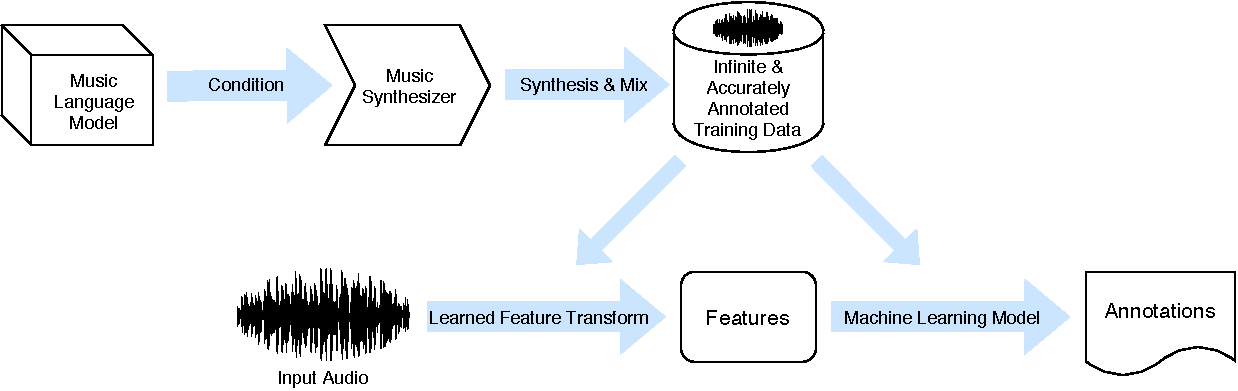
\includegraphics[width=\textwidth]{paradigms-5-proposed.pdf}
	\caption{A combination of music language model and music synthesizer can be used as an infinite source of accurately annotated training data for a transcription model.}\label{fig:unlimited-data}
\end{figure}

Data augmentation can provide additional improvement in most music analysis tasks~\cite{mcfee2015muda}, although it was not considered in the experiments in this thesis, in order to keep the narratives focused on the novel approaches being introduced in each chapter.
While the conventional methods such as time stretch and pitch shift can be used for the purpose of music data augmentation, expressive music language models and music synthesis models can provide more powerful means of enriching the distribution of music data for training a transcription model.
This idea is illustrated in Figure~\ref{fig:unlimited-data}; an unlimited source of training data can be created using a combination of a powerful music language model and a good music synthesizer.
This idea is particularly promising considering the incredible performance of the recent transformer-based language models~\cite{vaswani2017attention}, which have been shown to be also effective in producing coherent symbolic music \cite{huang2019transformer}.

More powerful computational hardware in the future will enable a longer context length to be used in larger transformer models, which suggests another intriguing future research direction to learn a music language model in the audio waveform domain.
This will help create a more expressive synthesizer component, which can be used to augmenting a music transcription model.
A compression method such as VQ-VAE~\cite{oord2017vqvae} would be helpful in allowing even longer context length to be used in such language model.

\begin{figure}[b!]
	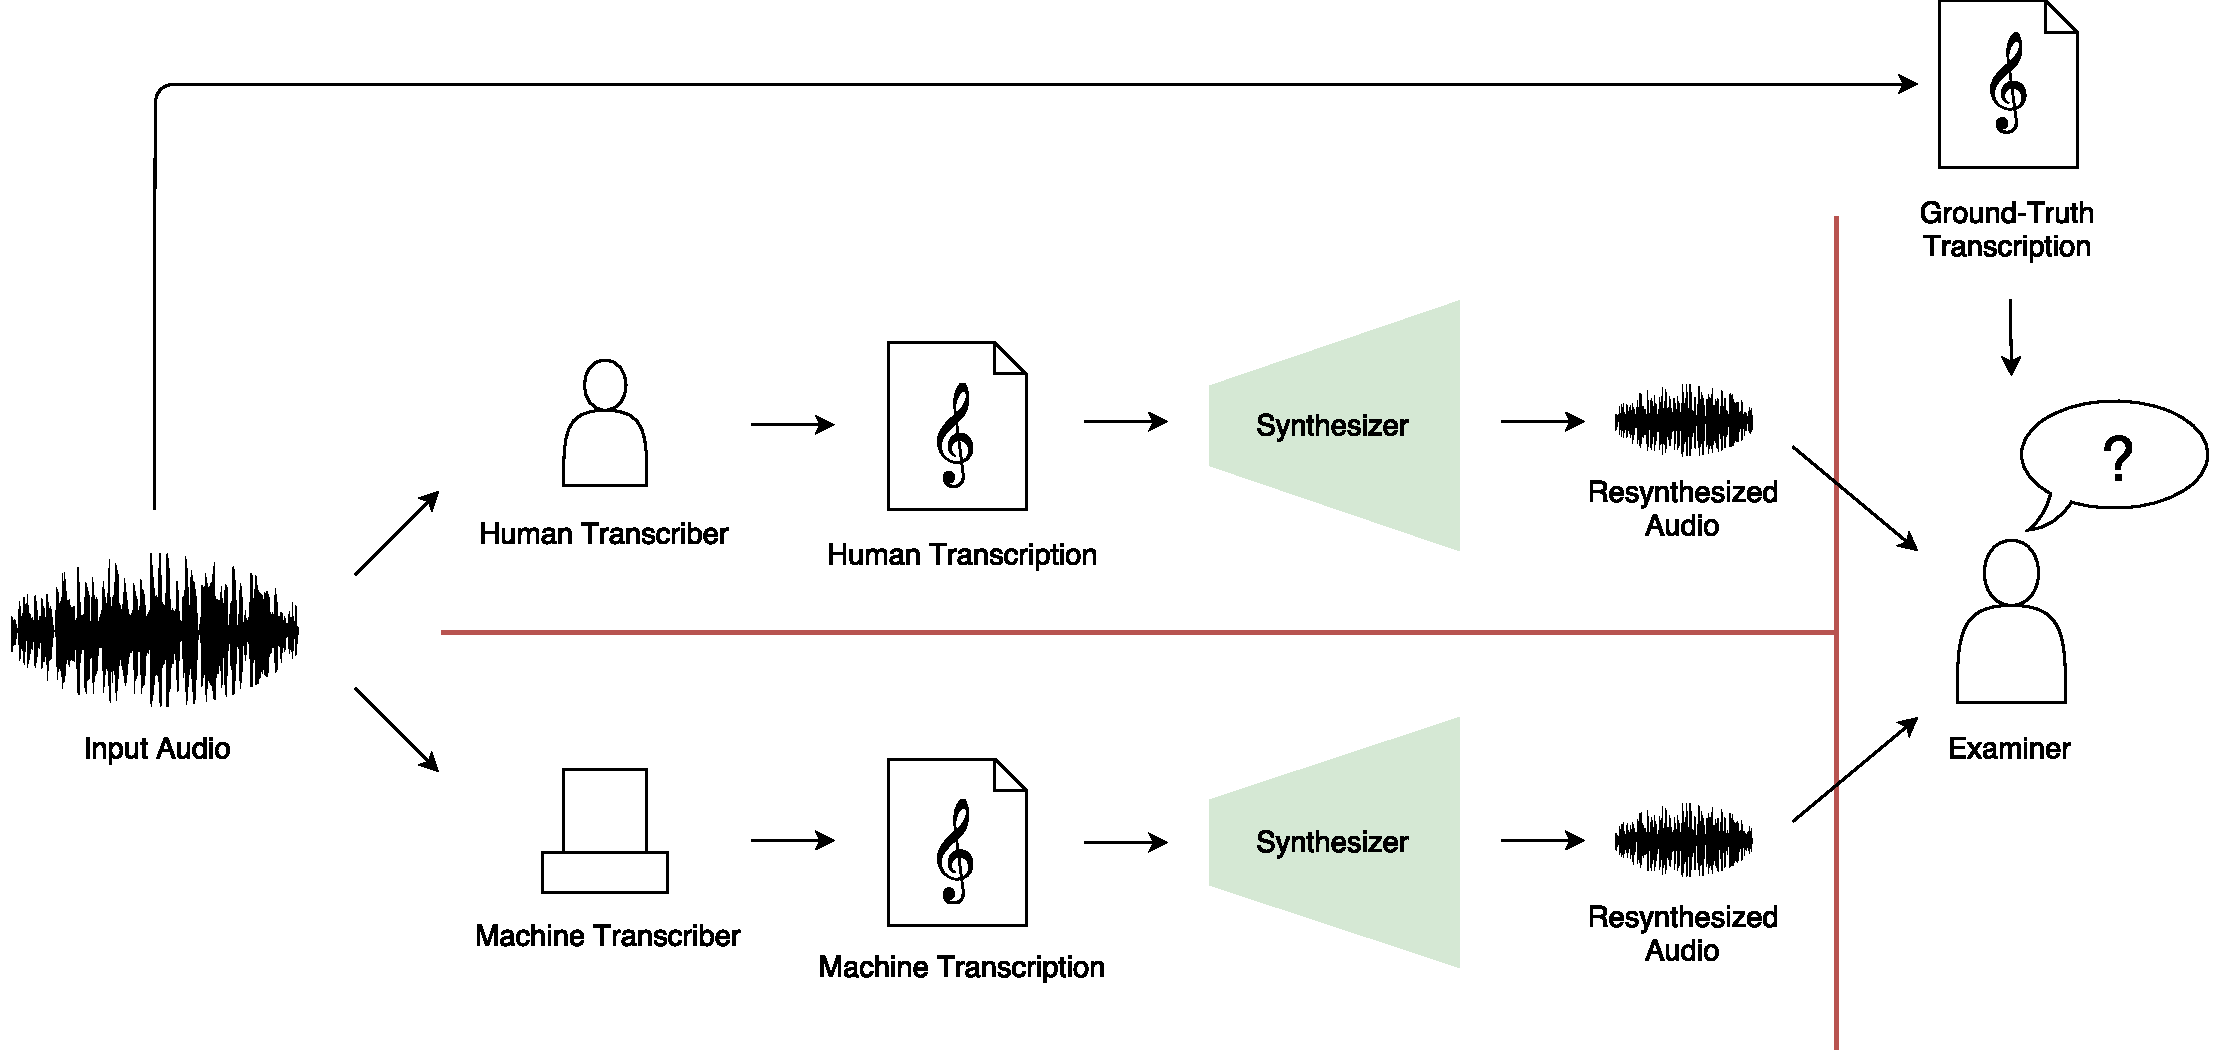
\includegraphics[width=\textwidth]{turing.pdf}
	\caption{The \emph{transcriptional Turing test}, to test whether an automatic music transcription algorithm has reached human-level. When an automatically generated transcription is indistinguishable by an expert human listener from one produced by a skilled musician, it can be said that AMT is solved.}
	\label{fig:turing}
\end{figure}


Finally, in the discussion regarding the future of AMT, we need to consider the fundamental limitation on any music transcription task, either automatic or manual, and when it can be said that AMT is solved.
Polyphonic music contains a mixture of sounds with an indefinite number of notes being played simultaneously; even the most experienced musicians may not be able to identify every note, and the audio mixture may not contain the sufficient information to convey all notes in the first place.
It would be unreasonable to expect anyone to perfectly transcribe all notes in the score of an orchestral music from an audio file, but it would be sensible for a trained musician to produce a version of score that, when played by the same orchestra, sounds indistinguishable to the original recording.
Considering these limitations, passing this ``transcriptional Turing test'' as shown in Figure \ref{fig:turing}, rather than achieving the 100\% accuracy on a certain dataset, should be the ultimate goal of automatic music transcription, at which point it can be said to have a human-level intelligence on this task.

So when will that happen? Considering the astounding success in the other `fooling humans department' in the recent years, all evidences suggest that the singularity is not too far in the future.

\pagebreak